% !TeX spellcheck = en_US
\documentclass[AMbeamer%               style
               ,optEnglish%            language
               %,handout%               deactivate animation
               ,optBibtex%              bibliography tool
               %,optBiber%               bibliography tool
               ,optBibstyleAlphabetic%
               ,optBeamerClassicFormat% 4:3 format
               %,optBeamerWideFormat%   16:9 format
               %,optExzellenz%
               ]{AMlatex}%
% \setbeameroption{show notes on second screen}% show notes}% Show all notes
%
%
% Tikz libraries
\usepackage{standalone}%
\usetikzlibrary{angles, arrows.meta, backgrounds, calc, decorations.pathmorphing, shapes.geometric, patterns, positioning, timeline, quotes}%
%
% Glossaries
\usepackage[acronyms, toc]{glossaries}
\makenoidxglossaries
\loadglsentries{source/glossary.tex} % important update for glossaries, before document
%
% Set paths
\graphicspath{{figures/}}%
\addbibresource{source/literature.bib}%
%
% Set meta data
% -------------
\title[Comparison of Controllers for Trunk Stabilization in a Bipedal Robot]{Comparison of Controllers for Trunk Stabilization in a Bipedal Robot}%
\def\PresentationType{\AMlangGerEng{Auftaktvortrag}{Initial Presentation}}%
%\def\PresentationType{\AMlangGerEng{Abschlussvortrag}{Final Presentation}}%
%\def\PresentationThesisType{\AMlangBachelorsThesis}%
%\def\PresentationThesisType{\AMlangSemesterThesis}%
\def\PresentationThesisType{\AMlangMastersThesis}%
%\def\PresentationThesisType{\AMlangInterdisciplinaryProject}%
\author[F. Schausberger]{Felix Schausberger}%
\def\PresentationExaminer{\AMnamesProfRixen}%
\def\PresentationSupervisor{Dr.-Ing. Daniel Renjewski}%
\date{\AMutilsDate{11}{10}{2022}}%%
%
% Setup of header and footer
\AMbeamerSetupHeader{\AMlayoutHeaderCustomChair}%
\AMbeamerSetupFooterCD%
%
\begin{document}%
%
% Start with titlepage
\AMbeamerTitlePageStudentThesis%
%
%
\begin{frame}{Introduction}%
    \begin{columns}[T,onlytextwidth]%
        \begin{column}[T]{0.48\textwidth}%
            \begin{enumerate}
                \item Objective: Stabilize torso
                \item Goal: Quantify correlations of parameters that influence periodic gait
                \item Implementation: Neural network controller, trajectory optimization,~\glsxtrlong{vlo}
                \item Evaluation:~\Glsxtrlong{mca}, stability analysis
            \end{enumerate}%
        \end{column}%
        \begin{column}[T]{0.48\textwidth}%
            \begin{figure}[htb]%
                \centering%
                \includegraphics[width=0.7\linewidth]{jenafox/jenafox-wireframe-transparent-black-thick.png}%
            \end{figure}%
        \end{column}%
    \end{columns}%
\end{frame}%
%%
\begin{frame}{Trajectory optimization~\cite{Rummel2010}~\cite{Renjewski2013}}%
    \begin{columns}[T,onlytextwidth]%
        \begin{column}[T]{0.5\textwidth}%
            \begin{figure}[htb]%
                \centering%
                \includestandalone{vlo/vlo}
            \end{figure}%
        \end{column}%
        \begin{column}[T]{0.35\textwidth}%
            \begin{figure}[htb]%
                \centering%
                \includegraphics[width=\textwidth]{jenafox/basic-coordinates.png}
            \end{figure}%
        \end{column}%
    \end{columns}%
    \begin{align}
        f &= \sum_{i = 3}^{7}~\lvert~q_i(\glsxtrshort{vlo}_1)~-~q_i(\glsxtrshort{vlo}_0)~\rvert~+~\lvert~\dot{q}_i(\glsxtrshort{vlo}_1)~-~\dot{q}_i(\glsxtrshort{vlo}_0)~\rvert \notag
    \end{align}
\end{frame}%
%%
\begin{frame}{Vertical leg orientation}%
    \begin{figure}[H]%
        \centering%
        \begin{subfigure}[t]{0.25\linewidth}%
            \centering%
            \includegraphics[width=\linewidth]{jenafox/vlo/vlo0.png}
            % \caption{\glsxtrshort{vlo}$_{0}$}%
            \label{fig:jenafox-vlo0}%
            % \vspace*{2mm}%
        \end{subfigure}%
        %
        \begin{subfigure}[t]{0.25\linewidth}%
            \centering%
            \includegraphics[width=\linewidth]{jenafox/vlo/vlo1.png}
            % \caption{Right hip\\flexion}%
            \label{fig:jenafox-vlo1}%
            \vspace*{2mm}%
        \end{subfigure}%
        %
        \begin{subfigure}[t]{0.25\linewidth}%
            \centering%
            \includegraphics[width=\linewidth]{jenafox/vlo/vlo2.png}
            % \caption{Right knee\\extension}%
            \label{fig:jenafox-vlo2}%
            \vspace*{2mm}%
        \end{subfigure}%
        %
        \begin{subfigure}[t]{0.25\linewidth}%
            \centering%
            \includegraphics[width=\linewidth]{jenafox/vlo/vlo3.png}
            % \caption{Double support}%
            \label{fig:jenafox-vlo3}%
            \vspace*{2mm}%
        \end{subfigure}%
        %
        \vfil
        %
        \begin{subfigure}[b]{0.25\linewidth}%
            \centering%
            \includegraphics[width=\linewidth]{jenafox/vlo/vlo4.png}
            % \caption{Left knee\\flexion}%
            \label{fig:jenafox-vlo4}%                      
        \end{subfigure}%
        %
        \begin{subfigure}[b]{0.25\linewidth}%
            \centering%
            \includegraphics[width=\linewidth]{jenafox/vlo/vlo5.png}
            % \caption{Right hip\\extension}%
            \label{fig:jenafox-vlo5}%                      
        \end{subfigure}%
        %
        \begin{subfigure}[b]{0.25\linewidth}%
            \centering%
            \includegraphics[width=\linewidth]{jenafox/vlo/vlo6.png}
            % \caption{Left hip\\flexion}%
            \label{fig:jenafox-vlo6}%                      
        \end{subfigure}%
        %
        \begin{subfigure}[b]{0.25\linewidth}%
            \centering%
            \includegraphics[width=\linewidth]{jenafox/vlo/vlo7.png}
            % \caption{\glsxtrshort{vlo}$_{1}$\newline}%
            \label{fig:jenafox-vlo7}%                      
        \end{subfigure}%
    \end{figure}%
    % \noindent
\end{frame}%
%%
\begin{frame}{Mechanical Cost Analysis~\cite{Lee2011}}%
    \begin{columns}[T,onlytextwidth]%
        \begin{column}[T]{0.5\textwidth}%
            \shorthandoff{"}% Needed for quotes
            $~\gls{phi} = \gls{lambda} + \gls{theta} \neq 0$:
            \begin{figure}[htb]%
                \centering%
                \includestandalone{mca/compliant-slip/compliant-slip}
                % \caption{Compliant~\glsxtrshort{slip} (\ie$~\gls{phi} = \gls{lambda} + \gls{theta} \neq 0$ and$~\gls{kappa} = 1$)}
            \end{figure}%
        \end{column}%
        \begin{column}[T]{0.5\textwidth}%
            \shorthandoff{"}% Needed for quotes
            $~\gls{phi} = \lvert\gls{lambda} - \gls{theta}\rvert = 0$:
            \begin{figure}[htb]%
                \centering%
                \includestandalone{mca/zero-collision/zero-collision}
                % \caption{Zero-collision (\ie$~\gls{phi} = \lvert\gls{lambda} - \gls{theta}\rvert = 0$ and$~\gls{kappa} = 0$)}
            \end{figure}%
        \end{column}%
    \end{columns}%
    \begin{align}
        \gls{phi} = \textrm{arcsin}\left(\frac{\vert\glsxtrshort{grf} \cdot \gls{v}_{\glsxtrshort{com}}\vert}{\vert\glsxtrshort{grf}\vert~\vert\gls{v}_{\glsxtrshort{com}}\vert}\right) \notag
    \end{align}
    \begin{align}
        \gls{lambda} = \textrm{arccos}\left(\frac{\vert\gls{v}_{\glsxtrshort{com}_x}\vert}{\vert\gls{v}_{\glsxtrshort{com}}\vert}\right),~
        \gls{theta} = \textrm{arccos}\left(\frac{\vert\glsxtrshort{grf}_y\vert}{\vert\glsxtrshort{grf}\vert}\right) \notag
    \end{align}
\end{frame}%
%%
\begin{frame}{Collision fraction~\cite{Lee2011}}%
    \begin{align}
        \gls{kappa} = \frac{\sum\vert\glsxtrshort{grf}\vert~\vert\gls{v}_{\glsxtrshort{com}}\vert~(\gls{phi} / (\gls{theta} + \gls{lambda}))}{\sum\vert\glsxtrshort{grf}\vert~\vert\gls{v}_{\glsxtrshort{com}}\vert} = \frac{\gls{Phi}}{\gls{Theta} + \gls{Lambda}} \notag
    \end{align}
    \begin{align}
        \gls{Phi} = \frac{\sum\vert\glsxtrshort{grf}\vert~\vert\gls{v}_{\glsxtrshort{com}}\vert~\gls{phi}}{\sum\vert\glsxtrshort{grf}\vert~\vert\gls{v}_{\glsxtrshort{com}}\vert} \notag
    \end{align}
    \begin{align}
        \gls{Lambda} = \frac{\sum\vert\gls{v}_{\glsxtrshort{com}}\vert~\gls{lambda}}{\sum\vert\gls{v}_{\glsxtrshort{com}}\vert} \notag
    \end{align}
    \begin{align}
        \gls{Theta} = \frac{\sum\vert\glsxtrshort{grf}\vert~\gls{theta}}{\sum\vert\glsxtrshort{grf}\vert} \notag
    \end{align}
    \begin{align}
        \gls{Phi} \approxeq \frac{\sum\vert\glsxtrshort{grf} \cdot \gls{v}_{\glsxtrshort{com}}\vert}{\sum\vert\glsxtrshort{grf}\vert~\vert\gls{v}_{\glsxtrshort{com}}\vert} \approxeq \text{\glsxtrshort{mcot}} = \frac{\sum\vert\glsxtrshort{grf} \cdot \gls{v}_{\glsxtrshort{com}}\vert}{\overline{\gls{v}_{\glsxtrshort{com}_x}}~\gls{m}~\gls{g}} \notag
    \end{align}
\end{frame}%
%%
\begin{frame}{Horizontal velocity}%
    \begin{figure}[htb]%
        \centering%
        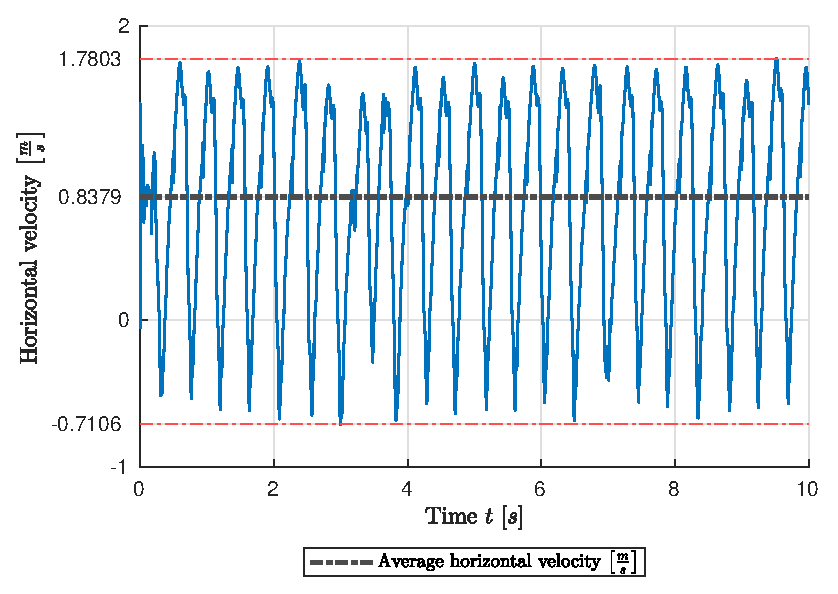
\includegraphics[width=0.8\textwidth]{com-horizontal-velocity/com-horizontal-velocity.eps}
    \end{figure}%
\end{frame}%
%%
\begin{frame}{Displacement}%
    \begin{columns}[T,onlytextwidth]%
        \begin{column}[T]{0.5\textwidth}%
            \begin{figure}[htb]%
                \centering%
                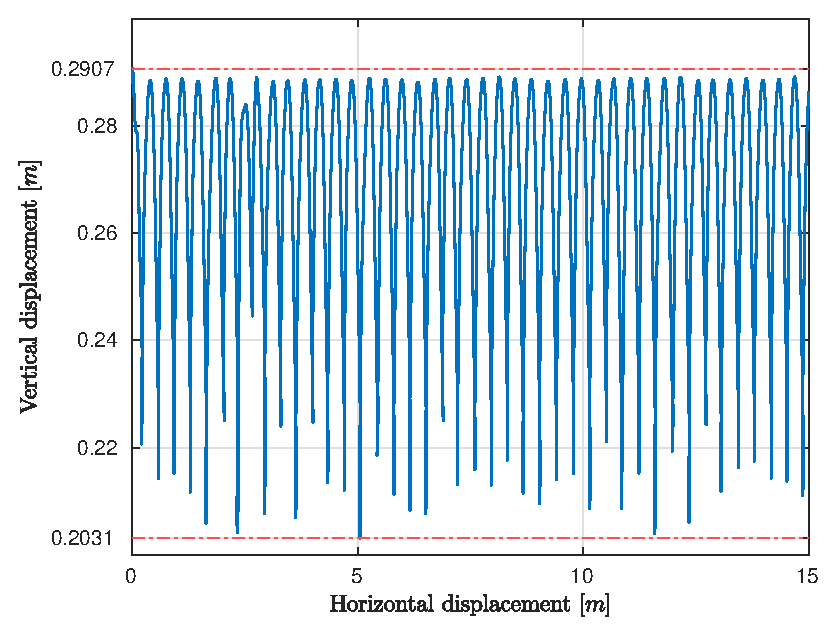
\includegraphics[width=\linewidth]{displacement/displacement.eps}
            \end{figure}%
        \end{column}%
        \begin{column}[T]{0.5\textwidth}%
            \begin{figure}[htb]%
                \centering%
                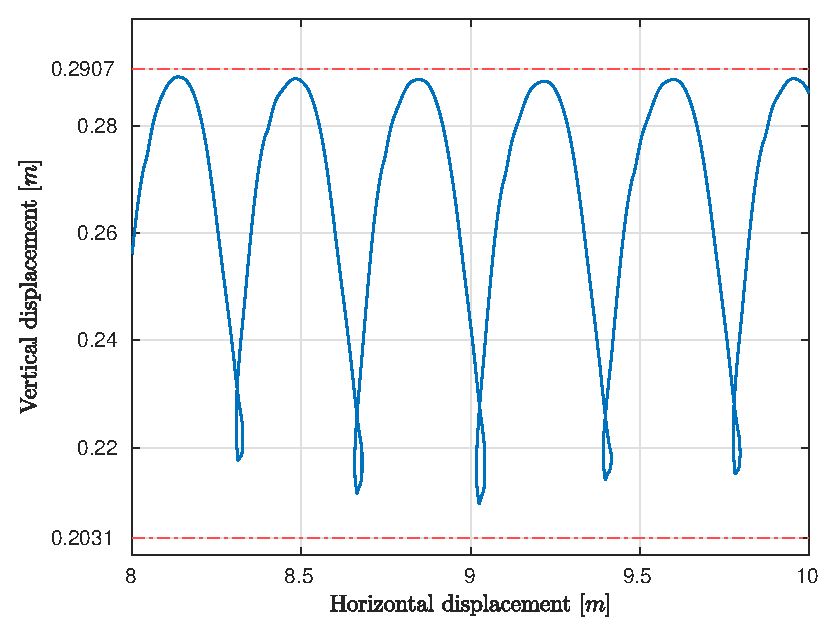
\includegraphics[width=\linewidth]{displacement/displacement-zoom.eps}  
            \end{figure}%
        \end{column}%
    \end{columns}%
\end{frame}%
%%
\begin{frame}{Torso and hip angle}%
    \begin{figure}[H]%
        \centering%
        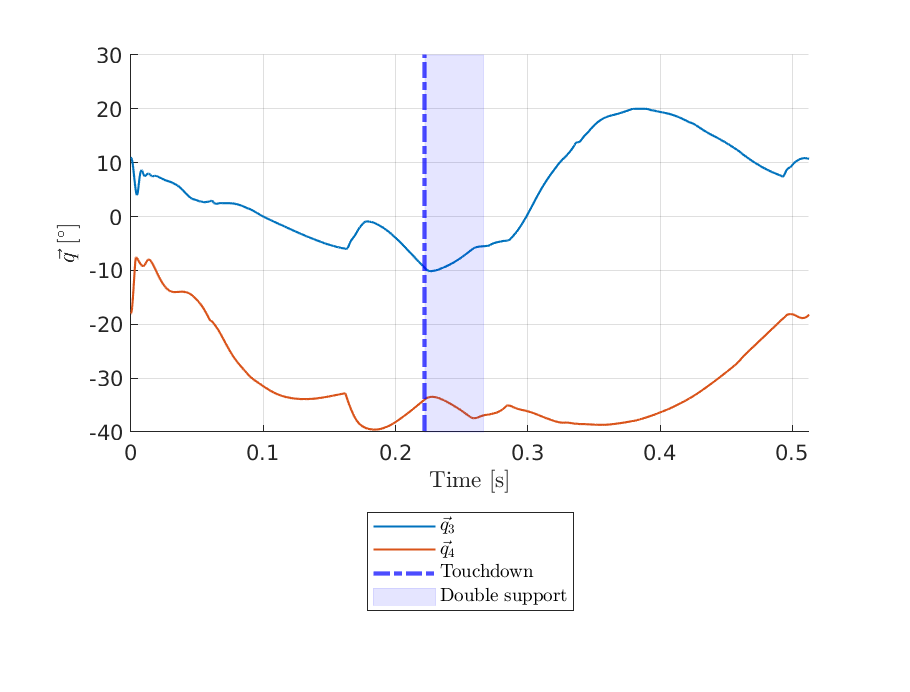
\includegraphics[width=0.8\linewidth]{phi-hip-torso/phi-hip-torso.eps}
    \end{figure}%
\end{frame}%
%%
\begin{frame}{Phase plot with ground-state}%
    \begin{figure}[htb]%
        \centering%
        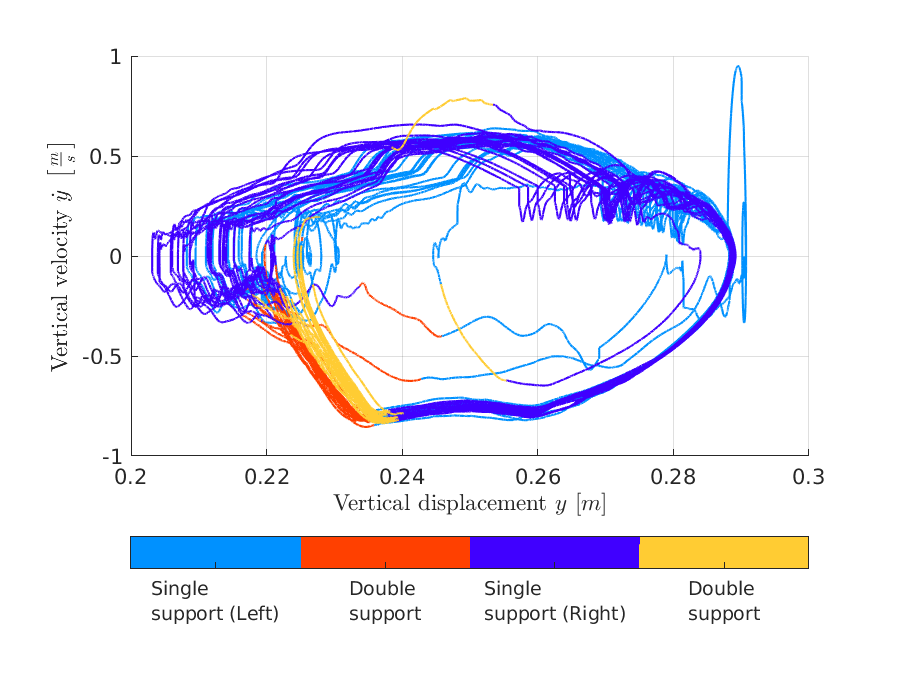
\includegraphics[width=0.75\textwidth]{phase-plot/phase-plot-ground-state.eps}
    \end{figure}%
\end{frame}%
%%
\begin{frame}{Phase plot with ground-state}%
    \begin{figure}[htb]%
        \centering%
        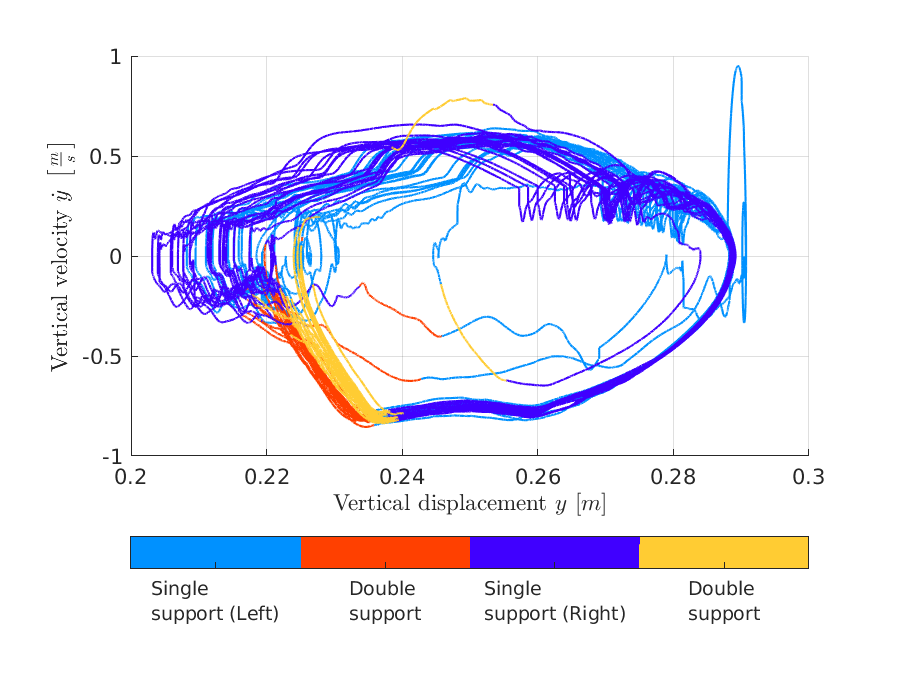
\includegraphics[width=0.75\textwidth]{phase-plot/phase-plot-ground-state.eps}
    \end{figure}%
\end{frame}%
%%
\begin{frame}{Summary}%
    \begin{columns}[T,onlytextwidth]%
        \begin{column}[T]{0.48\textwidth}%
            \begin{enumerate}
                \item Objective: Stabilize torso
                \item Goal: Quantify correlations of parameters that influence periodic gait
                \item Implementation: Neural network controller, trajectory optimization,~\glsxtrshort{vlo},~\glsxtrshort{mca}
                \item Result: Asymptotically stable gait found
                \item Evaluation: Not energy efficient
            \end{enumerate}%
        \end{column}%
        \begin{column}[T]{0.48\textwidth}%
            \begin{figure}[htb]%
                \centering%
                \includegraphics[width=0.7\linewidth]{jenafox/jenafox-wireframe-transparent-black-thick.png}%
            \end{figure}%
        \end{column}%
    \end{columns}%
\end{frame}%
%%

%
% End with titlepage
\AMbeamerTitlePageStudentThesis%
%
% Appendix
% \include{source/}%
\begin{frame}{Control parameters~\cite{Jenafox:ISB}}%
    \begin{figure}[H]% 
        \centering%
        \begin{subfigure}{0.5\linewidth}%
            \includegraphics[width=\linewidth]{jenafox/jenafox-ISB-convention-hip.png}
        \end{subfigure}%
        %
        \hfil%
        %
        \begin{subfigure}{0.5\linewidth}%
            \includegraphics[width=\linewidth]{jenafox/jenafox-ISB-convention-knee.png}
        \end{subfigure}%
    \end{figure}%
\end{frame}%
%%
\begin{frame}{Results}%
    \begin{align}
        \gls{theta-es}_{,~k} = -4.25 \notag
    \end{align}
    \begin{align}
        \gls{theta-fs}_{,~h} =~\text{\glsxtrshort{aea}} = \frac{15}{1 + e^{0.2 \cdot \gls{rho} + 4}} - 25 \notag
    \end{align}
    \begin{align}
        \gls{GM}_h = 1.6 \notag
    \end{align}
    \begin{figure}[H]%
        \centering%
        \includestandalone{mapping/sigmoid}
    \end{figure}%
\end{frame}%
%%
\begin{frame}{Results II}%
    \begin{center}
        \begin{tabular}{ l|l|l|l }
            \textbf{Symbol}                             & \textbf{Description}              & \textbf{Value}    & \textbf{Unit}                                     \\ [0.5ex]
            \hline \hline
            $\gls{x}_{\glsxtrshort{com},~end}$          & Distance covered                  & 15                &$~\left[\si{\metre}\right]$                        \\
            $\gls{t}_{end}$                             & Time required                     & 18.8502           &$~\left[\si{\second}\right]$                       \\
            $\overline{\gls{v}_{\glsxtrshort{com}_x}}$  & Average forward velocity          & 0.8379            &$~\left[\si{\metre\per\second}\right]$             \\
            $\gls{v}_{\glsxtrshort{com}_x,~max}$        & Maximum instantaneous velocity    & 1.7803            &$~\left[\si{\metre\per\second}\right]$             \\
            $\gls{v}_{\glsxtrshort{com}_x,~min}$        & Minimum instantaneous velocity    & -0.7106           &$~\left[\si{\metre\per\second}\right]$             \\
            $\gls{y}_{\glsxtrshort{com},~max}$          & Highest vertical displacement     & 0.2907            &$~\left[\si{\metre}\right]$                        \\
            $\gls{y}_{\glsxtrshort{com},~min}$          & Lowest vertical displacement      & 0.2031            &$~\left[\si{\metre}\right]$                        \\
            $\gls{Fr}$                                  & Froude number                     & 0.2468            & -                                                 \\
            $\sqrt{\gls{Fr}}$                           & Dimensionless velocity            & 0.4986            & -                                                 \\
            $\gls{Theta}$                               & Average force angle               & 0.7285            & $\left[\si{\radian}\right]$                       \\
            $\gls{Lambda}$                              & Average velocity angle            & 0.3704            & $\left[\si{\radian}\right]$                       \\
            $\gls{Phi}$                                 & Average collision angle           & 0.9855            & $\left[\si{\radian}\right]$                       \\
            \glsxtrshort{mcot}                          & \glsdesc{mcot}                    & 0.5226            & $\left[\si{\joule\per\metre\per\newton}\right]$   \\
            $\gls{kappa}$                               & Collision fraction                & 0.8968            & - 
        \end{tabular}
    \end{center}
\end{frame}%
%%
\begin{frame}{Velocity vectors}%
    \begin{columns}[T,onlytextwidth]%
        \begin{column}[T]{0.5\textwidth}%
            \begin{figure}[htb]%
                \centering%
                \includegraphics[width=\linewidth]{velocity-vectors/touchdown/velocity-vectors-touchdown.eps}
            \end{figure}%
        \end{column}%
        \begin{column}[T]{0.5\textwidth}%
            \begin{figure}[htb]%
                \centering%
                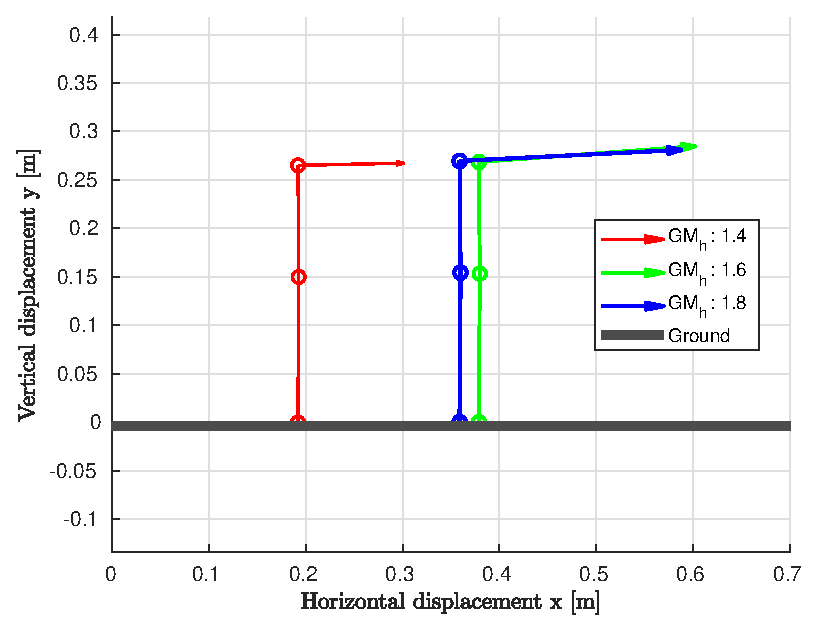
\includegraphics[width=\textwidth]{velocity-vectors/vlo/velocity-vectors-vlo.eps}
            \end{figure}%
        \end{column}%
    \end{columns}%
\end{frame}%
%%
%
% References
\AMbeamerSetFooterText{References}%
\begin{frame}[allowframebreaks]{References}%
    %\sloppy% "Word"-like typesetting in order to improve breaking lines with long URLs/DOIs
    \printbibliography[heading=none]%
\end{frame}%
%%
%
% Glossary
\AMbeamerSetFooterText{Glossary}%
\begin{frame}[allowframebreaks]{Glossary}%
    \printnoidxglossaries%
\end{frame}%
%
\end{document}%
%
%
